
This experiment explored the consequences of varying the agent's sensor model parameters while keeping all other parameters at their default values, outlined in Section \ref{sec:SimulationResults}. We varied the FPR and FNR of the agent's sensor model to reflect the cases where they underestimate (FPR=0.05, FNR=0.02), correctly estimate (FPR=0.2, FNR=0.15) and overestimate (FPR=0.05, FNR=0.02) the correct rates at which the sensor will record false positive and false negative observations. The correct rate at which the sensor makes false negative and false positive observations was set for all experiments as 0.2 and 0.15 respectively.




\begin{table}[H]
    \centering
    \begin{tabular}{| >{\centering} m{18mm} | >{\centering}m{15mm} | >{\centering}m{15mm} | >{\centering}m{18mm} | >{\centering}m{18mm} | >{\centering}m{18mm} | m{19mm} <{\centering}|}
    \hline
       Strategy & Sensor Model FPR & Sensor Model FNR & Mean TTD & Sample SD[TTD] & False Negative Rate & Proportion Incorrectly Localised \\
        \hline
        $\epsilon$-Greedy & 0.05 & 0.02 & 67.2488 & 43.2448 & 0.1368 & 0.4270 \\
        $\epsilon$-Greedy & 0.2 & 0.15 & 112.9258 & 62.3798 & 0.1516 & 0.0398 \\
        $\epsilon$-Greedy & 0.4 & 0.4 & 197.5886 & 113.1707 & 0.0008 & 0.0000 \\
        \hline

        Saccadic & 0.05 & 0.02 & 59.9230 & 38.6500 & 0.1440 & 0.4298 \\
        Saccadic & 0.2 & 0.15 & 98.8274 & 56.1298 & 0.1588 & 0.0370 \\
        Saccadic & 0.4 & 0.4 & 142.2648 & 96.2213 & 0.0006 & 0.0 \\
        \hline
        
        Random & 0.05 & 0.02 & 167.2306 & 134.0652 & 0.015 & 0.7044 \\
        Random & 0.2 & 0.15 & 629.5462 & 282.9514 & 0.1368 & 0.0366 \\
        Random & 0.4 & 0.4 & 2100.5140 & 659.7263 & 0.1682 & 0.0 \\
        \hline
        
        Sweep & 0.05 & 0.02 & 132.1120 & 74.3178 & 0.0162 & 0.7932 \\
        Sweep & 0.2 & 0.15 & 601.5697 & 183.4529 & 0.1254 & 0.0454 \\
        Sweep & 0.4 & 0.4 & 2138.6002 & 554.5915 & 0.1344 & 0.0 \\
        \hline
        
    \end{tabular}

  \caption{Results of running the target localisation simulation with varying sensor model parameters for each implemented search strategy.}
  \label{table:MiscalibratedSensor}
\end{table}


Table \ref{table:MiscalibratedSensor} displays the results of running a simulation with a single agent and a single target while varying the parameters of the sensor model. The sensor model is parameterised using a false positive rate and false negative rate, detailed in equation \ref{eqn:EvidenceVarsProbs}. For this set of simulations, we deliberately chose extreme values for these parameters to show the effects of an extreme miscalibration, which can be thought of as a worst case scenario. We discuss the results in terms of underestimating and overestimating the true sensor parameters:
\begin{enumerate}
    \item When the model is calibrated to underestimate the rate at which the sensor will detect false negatives and false positives (the rows which have a sensor model FPR = 0.05, sensor model FPR = 0.02 in Table \ref{table:MiscalibratedSensor}), relative to the correctly calibrated sensor model (the rows which have a sensor model FPR = 0.2, sensor model FPR = 0.15 in Table \ref{table:MiscalibratedSensor}), both positive and negative observations will have a greater effect on the change in the shape of the distribution of the agent's belief, since the sensor model is more confident that the readings are correct. This means that is easier to cross the decision threshold of the SPRT due to spurious observations. For example, it would require 3, 5 and 17 positive consecutive observations at the same location to cross the upper SPRT threshold in the cases that the sensor model is calibrated with FPR=0.05/FPR=0.02, FPR=0.2/FPR=0.15, FPR=0.4/FPR=0.4 respectively.
    \par Underestimating the true sensor parameters leads to a much higher incorrect localisation rate in the adaptive search strategies in relation to the non-adaptive search strategies, which is evident in the Proportion Incorrectly Localised column of Table \ref{table:MiscalibratedSensor}. The reason for this is that the non-adaptive search strategies do not follow up on positive observations. The agent belief increases a relatively large amount with every positive observation, which actually arrive at a much higher rate (0.2066) than the sensor is calibrated for (0.0593). For example, if the agent immediately makes a positive observation, its belief will jump from 0.5 to 0.5425. Figure \ref{fig:MiscalibratedSensorFPR005} (a) shows the evolution of the agent's cumulative belief that the target is present in the search region. Relatively large jumps in cumulative belief due to the miscalibrated sensor model are clearly visible. This is in contrast with the adaptive strategies, where the agent re-samples positive observations, which drives the agent's belief back down in the case of spurious positives, which is visible in Figure \ref{fig:MiscalibratedSensorFPR005} (b).
    
    %\textit{Proportion Incorrectly Localised} column of table \ref{table:MiscalibratedSensor}. Similarly, we see that the false negative rate increases, as the miscalibrated model causes the belief in the target being absent for the region to increase more sharply with negative observations than the correctly calibrated sensor model. The mean time to decision (TTD) increases in this case because the belief in the target presence jumps disproportionately when a positive observation is made relative to a negative observation. The ratio of the sensor model FPR to FNR is approximately half the true ratio, which means the effect of positive observations is underestimated, causing the agent to delay the conclusion in a positive target localisation.
    \item Conversely, when the model is calibrated to overestimate the rate at which the sensor will record false positives and false negatives (the rows which have a sensor model fpr = 0.4, sensor model FPR = 0.4 in Table \ref{table:MiscalibratedSensor}), the belief distribution changes much more gradually given positive or negative observations. This means that crossing the decision thresholds given by the SPRT will require many more positive or negative readings, which leads to much higher mean times to decision (TTD) for all search strategies. As a lower bound, the SPRT would require 447 consecutive negative observations when running the sweep search in order to conclude that the target is not present. In the adaptive cases, once a positive observation is made at a given location, the agent's belief usually becomes highest at that location, which causes the agent to sample there again. Once it visits the true target location, usually it will receive a sufficient number of positive observations to keep sampling it, which causes its cumulative belief to steadily increase, as shown in Figure \ref{fig:MiscalibratedSensorFPR04} (a). The non-adaptive methods do not exhibit this behaviour since they are unbiased sampling methods. They do not re-sample when they come across a positive observation, which causes their cumulative belief that the target is present to gradually drop. If they do not experience consecutive positive observations when they visit the true target location, usually their belief will drop below the SPRT threshold, as can be seen in Figure \ref{fig:MiscalibratedSensorFPR04} (b).
\end{enumerate}

\begin{figure}[H]
\centering
    \subfloat[Sample run using Sweep search strategy]{{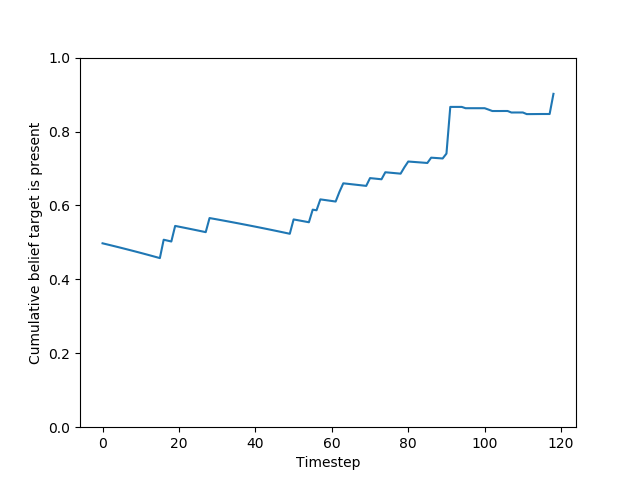
\includegraphics[width=7.5cm]{Chapters/MultiAgentTargetDetection/Figs/Results/BeliefEvolution/MiscalibratedSensor/05-02/SweepBeliefEvolution4.png}}}%
    %\qquad
    \subfloat[Sample run using Saccadic search strategy]{{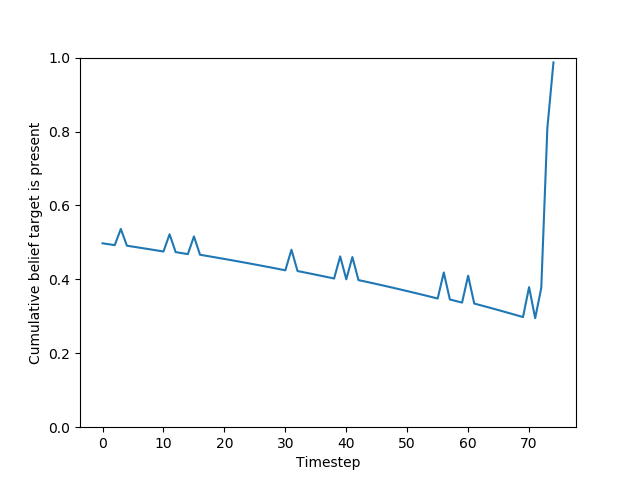
\includegraphics[width=7.5cm]{Chapters/MultiAgentTargetDetection/Figs/Results/BeliefEvolution/MiscalibratedSensor/05-02/SaccadicBeliefEvolution4.png} }}%
    \caption{Sample runs with miscalibrated sensor model parameters FPR=0.05, FNR=0.02}%
    \label{fig:MiscalibratedSensorFPR005}%
\end{figure}

\begin{figure}[H]
\centering
    \subfloat[Sample run using Random search strategy]{{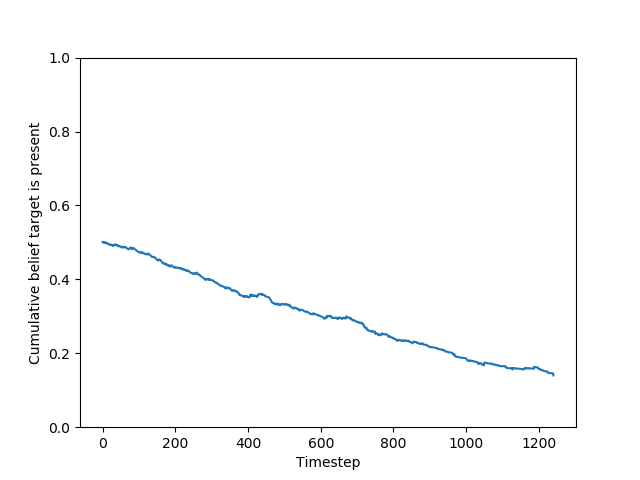
\includegraphics[width=7.5cm]{Chapters/MultiAgentTargetDetection/Figs/Results/BeliefEvolution/MiscalibratedSensor/4-4/RandomBeliefEvolution2.png}}}%
    %\qquad
    \subfloat[Sample run using Saccadic search strategy]{{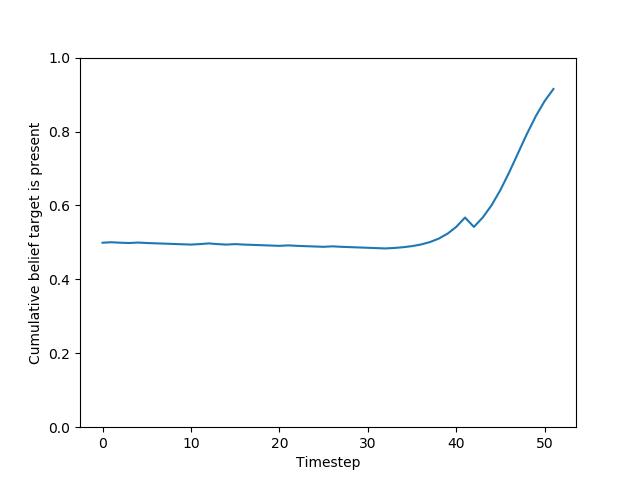
\includegraphics[width=7.5cm]{Chapters/MultiAgentTargetDetection/Figs/Results/BeliefEvolution/MiscalibratedSensor/4-4/SaccadicBeliefEvolution0.png} }}%
    \caption{Sample runs with miscalibrated sensor model parameters FPR=0.4, FNR=0.4}%
    \label{fig:MiscalibratedSensorFPR04}%
\end{figure}